\documentclass{article}
\usepackage{tikz}
\usetikzlibrary{shapes.geometric}

\begin{document}

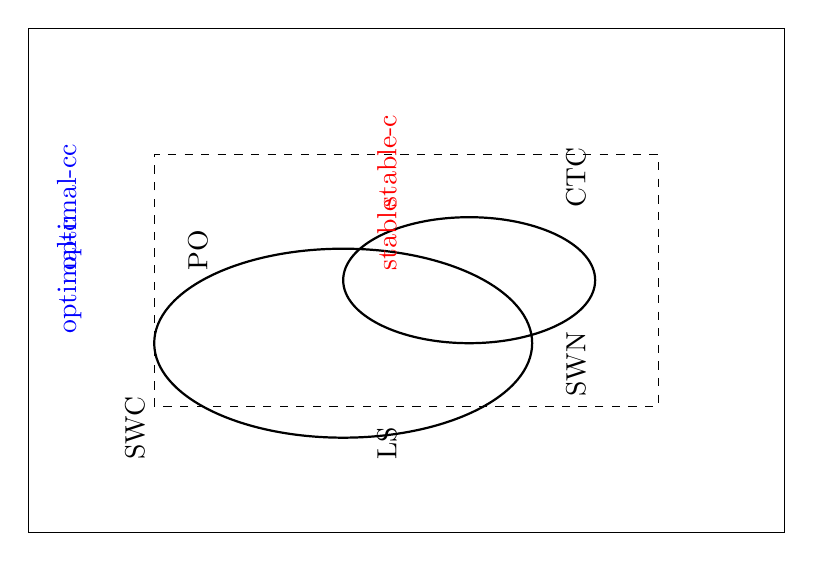
\begin{tikzpicture}[scale=0.8]
    % Draw the outer rectangle
    \draw (0,0) rectangle (12,8);
    
    % Draw the inner rectangle
    \draw[dashed] (2,2) rectangle (10,6);
    
    % Draw the ellipse
    \draw[thick] (5,3) ellipse (3cm and 1.5cm);
    
    % Draw the smaller ellipse
    \draw[thick] (7,4) ellipse (2cm and 1cm);
    
    % Label the regions
    \node at (1,4) [anchor=south west, rotate=90] {\textcolor{blue}{optimal-cc}};
    \node at (1,3) [anchor=south west, rotate=90] {\textcolor{blue}{optimal-c}};
    \node at (3,4) [anchor=south west, rotate=90] {PO};
    \node at (6,5) [anchor=south west, rotate=90] {\textcolor{red}{stable-c}};
    \node at (6,4) [anchor=south west, rotate=90] {\textcolor{red}{stable}};
    \node at (9,5) [anchor=south west, rotate=90] {CTC};
    \node at (9,2) [anchor=south west, rotate=90] {SWN};
    \node at (6,1) [anchor=south west, rotate=90] {LS};
    \node at (2,1) [anchor=south west, rotate=90] {SWC};
\end{tikzpicture}

\end{document}